\documentclass[runningheads]{llncs}

\input{settings}

\title{Modular IDE}

\author{Nils Michael Fitjar\inst{1,2}}

\authorrunning{Nils Michael Fitjar}

\institute{Western Norway University of Applied Sciences\\
\email{798183@stud.hvl.no}
\and
University of Bergen\\
\email{nfi005@uib.no}
}

\begin{document}

\frontmatter

\maketitle

\chapter{Abstract} \label{abstract}

\begin{abstract}
  This paper introduces a Modular, \textit{Zero Core}, Application, to serve as
  an Integrated Development Environment (IDE) for experimental programming
  languages, addressing limitations in traditional IDEs. While standard IDEs are
  crucial in software development, their support for experimental languages is
  often inadequate. This can and, has been solved by extensively using the
  plugin/module architecture of existing IDEs. However, relying on
  \textit{niche} plugins/functionality is not future safe.
  % TODO: Rewrite this sentence
  This project proposes a modular IDE to extend its lifespan and enhance support
  for experimental languages. Analyzing the essential features of traditional
  IDEs and the need for adaptability to new paradigms and tools. Magnolia, a
  research programming language developed at UIB, serves as a case study,
  highlighting its unique characteristics and the necessity for a specialized
  IDE. The primary research question explores how modularization facilitates the
  design and implementation of experimental programming languages. Specific
  modules tailored for experimental languages, including Abstract Semantic
  Representation (ASR) Transformation, Term Algebras, MoA translation, and
  Syntactic Theory Functor (STF), are outlined. To showcase the usefulness of
  a modular approach, the modules needed to extend the core application to an
  IDE will be implemented.
  \keywords{Modularization \and IDE \and Magnolia.}
\end{abstract}

\tableofcontents

\mainmatter

\chapter{Introduction} \label{ch:intro}
\chapter{Introduction}

Standard \gls{ide}s are indispensable tools in software development, offering features
like early bug reporting, project outline visualization, code highlighting, and
code completion However, these \gls{ide}s may not adequately support the unique
demands of experimental programming languages.
% Rewrite this
To solve this, a modular approach is used to designed and \gls{ide}.

\section{Experimental Languages}

Talk about Abstract Semantic Representation (ASR) Transformation,
Term Algebras, Mathematics of Arrays, and Syntactic Theory Functor (STF)

\section{Integrated Development Environment}

\todo{Rewrite this}
An \gls{ide}, aids a developer, as all the
needed tools for development are integrated into one application. There are
different kinds of \gls{ide}, generic and specialized.

A specialized \gls{ide} is one targeted towards a specific language, like Eclipse,
(reference?), or IntelliJ (reference?), which target Java/JVM. It contains
specialized features like:

\begin{itemize}
  \item Syntax Highlighting
  \item Code Autocompletion
  \item Go-to-definitions
  \item \dots
\end{itemize}

A lot of these features are possible due to \textit{Language Server Protocols},
which allow for a standardized way for compilers to give code-support to \gls{ide}'s.

\todo{Connect these better}

A generic \gls{ide} contains the features that are common among development in any
programming language, like:

\todo{Should write a paragraph or two about each of these points}
\begin{itemize}
  \item File explorer
  \item Project manager
  \item Version Control System integration
\end{itemize}


\chapter{Background} \label{ch:background}
\chapter{Background}

\section{Magnolia}

Magnolia is an experimental research language being developed \gls{bldl} at the
University of Bergen. Magnolia is designed to support a high level of abstraction
and ease of reasoning. This is achieved by \textit{concepts}, \textit{axioms} and
\textit{implementations}.

\todo{
  Add some reason for this way of thinking, with an example of real usage of
  semigroups, like some kind of API
}

Sets with specific operations acting on those elements, known as algebraic
structures, showcase the usage of concepts. Magma consists of a set with just a
singular binary operation, that must be closed by definition. A semigroup is an
extension of magma, with the added property that the binary operation is
associative. A monoid is an extension of a semigroup, with the added property
wherein an element in the set, \textit{C}, sometimes called a \textit{unit}, or
the \textit{identity}. This \textit{identity} ensures the following equation
holds, where the binary operation is $ \oplus $, and $ a, C $ are elements of the set.

\begin{equation}
  a \oplus C = a
\end{equation}

This, again, can be extended with an additional property, namely,
\textit{inverse element}.

\begin{equation}
  \forall a, \exists b, \in M \implies a \oplus b = C
\end{equation}

Assuming associativity.

This structure could be implemented in something like Java, an Object-Oriented
Language, as shown in listings \ref{lst:jmagma}, \ref{lst:jsemigroup},
\ref{lst:jmonoid}, and \ref{lst:jgroup}. Note the empty interfaces; there is
nothing that enforces the different laws on the properties. This can only be
done by unit testing, which is not enforced on a consumer of the \gls{api}.

\begin{center}
  \lstinputlisting
    [ language=Java
    , caption={Magma concept in Java}
    , label=lst:jmagma]{./code/magma.java}
\end{center}

\begin{center}
  \lstinputlisting
    [ language=Java
    , caption={Semigroup concept in Java, can only be upheld using unit tests}
    , label=lst:jsemigroup]{./code/semigroup.java}
\end{center}

\begin{center}
  \lstinputlisting
    [ language=Java
    , caption={Monoid concept in Java, can only be upheld using unit tests}
    , label=lst:jmonoid]{./code/monoid.java}
\end{center}

\begin{center}
  \lstinputlisting
    [ language=Java
    , caption={Group concept in Java, can only be upheld using unit tests}
    , label=lst:jgroup]{./code/group.java}
\end{center}

In Magnolia, however, this can be enforced on the \textit{interface}-level. The
example code shown in listing \ref{lst:magma}, showcases a concept
representation a binary operation, which has one function, \textit{magma}, which
takes in two values of type \textit{T}, and returns \textit{T}. Note that the
actual implementation of this function is missing. This is because a concept
encodes the properties of a users code. The actual implementation of the
\textit{magma} function needs to uphold the properties of the concept that is
being implemented. In this case, it is just that the input and output
of the function are of the same types.

\begin{center}
  \lstinputlisting
    [ language=Magnolia
    , caption={Magma concept in Magnolia}
    , label=lst:magma]{./code/magma.mg}
\end{center}

In the example code shown in listing \ref{lst:semigroup}, the \textit{magma}
concept has been expanded upon, still following the same rules as before, but
with the added property of associativity.

\begin{center}
  \lstinputlisting
    [ language=Magnolia
    , caption={Semigroup concept in Magnolia}
    , label=lst:semigroup]{./code/semigroup.mg}
\end{center}

\begin{center}
  \lstinputlisting
    [ language=Magnolia
    , caption={Monoid concept in Magnolia}
    , label=lst:monoid]{./code/monoid.mg}
\end{center}

\begin{center}
  \lstinputlisting
    [ language=Magnolia
    , caption={Group concept in Magnolia}
    , label=lst:group]{./code/group.mg}
\end{center}

\section{Reusable Software}

\subsection{Reuse in Magnolia}

\subsection{Software Lifetimes}

Software in general, lasts around 30 years (source). This is quite a long time,
but, this statistic is about more \textit{rigid} applications, which have an
unchanging scope. In more \textit{chaotic} fields, this number is reduced, as
paradigm shifts within certain fields, which results in the need for drastic
changes in the existing applications, where the needed work to change the code,
can be more than to create a new application.

\subsection{Software Longevity}

Most examples of \textit{popular} software, are open source, like \gls{vim}.
\gls{vim} is a text editor which has been in use since 1991. There are several
factors behind this success, but the ones being highlighted here, are due to its
extensibility and due to it being open-sourced. Being open sourced, allows for a
rotating cast of maintainers, ensuring the core application has the features its
users wants. The users of \gls{vim} can be split into two categories,
\textit{standard users}, and \textit{plugin developers}. \gls{vim} has an
extensive plugin ecosystem, which can extend \gls{vim}s functionality from a
text editor, to a fully fledged \gls{ide}.

\section{Integrated Development Environment}

An \gls{ide}, aids a developer, as all the needed tools for development are
integrated into one application. There are two different kinds of \gls{ide}s,
generic and specialized. \todo{Source}

A specialized \gls{ide} is one targeted towards a specific language, like
Eclipse, (reference?), or IntelliJ (reference?), which target Java/JVM. It
contains specialized features like the following:

\paragraph{Syntax Highlighting} Highlighting important keywords, identifiers
and more, makes the language easier to read for the developer, allowing them to
spot easy to miss errors, like misspelling of keywords.

\paragraph{Code Autocompletion} Suggesting keywords, method names or even entire
code snippets, is a powerful tool an \gls{ide} can have. This is possible to
achieve, in some form, without being specialized, by for example, suggesting
text that already exist in the document, but is most useful if it is
specialized, and can suggest built-in methods. This allows a developer to not
having to remember exactly how methods are named, is the method to split a
string by some delimiter, \textit{split\_by} or \textit{split\_on}? As long as
the developer writes \textit{split}, the correct method name will be suggested.

\paragraph{Go-To-Definitions} Being able to quickly navigate to methods and read
their implementation is a useful tool for a developer, as less time has to be
spent navigating the project structure, to figure out where some method was
implemented, and more time can be spent actually developing.

A lot of these features are possible due to \textit{Language Server Protocols},
which allow for a standardized way for compilers to give code-support to
\gls{ide}'s.

A generic \gls{ide} contains the features that are common among development in
any programming language, like:

\paragraph{File Explorer} Most project nowadays is larger than one file, so
being able to visualize the project in a tree-like-structure, and navigate that,
is useful. This feature usually comes with the ability to manipulate the project
structure, by adding files, folders, moving files around, and deleting them.

But creating any \gls{ide} would still limit the lifetime of the application.
The best example of a long living active \gls{ide}, or, at least editor, is Vim
(source?). Vim is not a feature full editor, but it is simple, lightweight, and
works on any operating system. But most people use it, for how easy it is to
extend; Its lifetime has been greatly extended by the ease of modularization.
Any popular module for Vim is open-source, and therefore, if any module had an
active community around it, if the \textit{lead} developer of the module stopped
developing it, that community can continue to develop the module, either by
getting maintenance access to the repository, or by forking it. Ensuring the
lifetime of the module is extended.

\subsection{Module Architecture}

\todo{Talk about modules in IDEs}

\todo{Find a way to mention this?}
\paragraph{Language Agnostic} The largest limiting factor in module oriented
applications, is the \textit{language barrier} Most applications limit what
language one can extend an application with, like in "Visual Studio Code", where
its JavaScript/HTML/CSS. Or IntelliJ, where one can use Java or Kotlin. But what
does language agnostic mean in the context of programming languages? It is, and
always will be C. Any \textit{serious} language can create some bindings with C.
So, for a module application to be Language Agnostic, it must be able to use C
Modules. This just means that the application must be able to call function from
a C library.

\subsection{Language Workbench}
\todo{Expand}
I don't know what this is.

\subsection{Language Server}

The most important features in a modern \gls{ide} are possible due to the
\gls{lsp}. \gls{lsp} is a protocol for a language server and editor,
(the client), with which they communicate, allowing for features like code
completion, syntax highlighting, marking of warnings and errors, as well as
refactoring routines. This client-server architecture, in \gls{ide}s are a
more recent development (2020s), as previously, support for the features
mentioned, were only possible due to specific modules being written for
specific \gls{ide}s. \gls{lsp} being the norm, is a sign of modularity being
preferred, as now a single \gls{lsp} can be created, and used across several
different applications, like IntelliJ, VS Code and Vim. While useful for
\textit{standard} language, this is the limiting factor when it comes to
supporting experimental languages, as not only does a new set of protocols need
to be appended to a language server, the editor itself needs to be changed to
actually use these protocols. This creates a lot of work, for both the \gls{ide}
developer and for the compiler developer. Here is where a modular approach can
help both. If some new functionality or feature is added to the experimental
language, this off course means the compiler/interpreter has to be expanded
and/or modified, but for the \gls{ide}, a module could be added/modified to
utilize this change, instead of having to change the entire application.

In this paper, we will start by discussing some background around modularity,
software longevity, and Magnolia (chapter 2). We will also discuss the different
ways to achieve modularity within an application, and point out different
behaviors that arise from such a setup (chapter 4). Finally, we will discuss the
results (chapter 5), and conclusions (chapter 6).

Traditional \gls{ide}s encompass essential features such as syntax highlighting, code
navigation, and hover-help, playing a crucial role in the software development
process. However, their limitations become apparent when working with
experimental languages. This paper advocates for modularization and
\textit{composability} as key design principles, demonstrating their ability to
extend the operational lifespan of software by allowing for ease-of adoption to
new paradigms and tools. The discussion revolves around Magnolia, an
experimental research programming language developed by \gls{bldl} at the
University of Bergen. Magnolia will act as a case study illustrating the need for
a specialized \gls{ide}. It is a way to experiment with novel language features.
And to achieve this in a sufficient manner, a more specialized \gls{ide} is
required.


\section{Existing Magnolia IDE}

The current \gls{ide} for Magnolia, is a many-years-old version of Eclipse,
using modules and functionality from the core Eclipse application, that has
since been outdated. The \gls{ide}s lifetime was limited by a dependency on
external modules and features that where not maintained by \gls{bldl}. This
meant that for future development of Magnolia, an outdated \gls{ide} was needed,
with outdated tooling. Furthermore, the Magnolia compiler was implemented as an
Eclipse module, which means that development is limited to Eclipse, and only
Eclipse, as a developer cannot compile Magnolia code without it.

Having the entire application available \textit{in-house}, will also help, as
open source; availability to the source code helps when developing niche
modules.

Modularization will help to mitigate some of the issues with the current
Magnolia \gls{ide}. Instead of maintaining an entire application, the needed and
wanted features of the application can be maintained instead.

Experimental languages might have features which are not possible to be fully
used in current \gls{ide}s. This is also the case for the current Magnolia
\gls{ide}. The compiler for Magnolia, syntax highlighting, error reporting, and
hover-functionality are functionality made in the Eclipse \gls{ide}, by using
its plug-in architecture. Some of the functionality and plug-ins this
implementation used, have been deprecated in later version of Eclipse. This
means the Magnolia \gls{ide} is locked to an old version of Eclipse, which, as
time passes, increases the complexity of installation, as the surrounding
tooling and libraries needed by this version of Eclipse also becomes deprecated.
Currently, in INF220, at the university, two weeks are set aside for students to
be able to install it.

\todo{Reference Anya's paper}


\section{Research questions}

\todo{Rewrite this}
Exploring how modularization can facilitate the design and implementation of
an integrated development environment targeting experimental programming
languages.

\todo{Red-thread is missing, find it}

\todo{Should probably also expand on what we mean by limiting (i.e. limiting in the sense of plugins being developed)}

\todo{Rewrite to be more academic enough}

\paragraph{Language Agnostic} The largest limiting factor in module oriented
applications, is the \textit{language barrier} Most applications limit what
language one can extend an application with, like in "Visual Studio Code", where
it's \textit{just} JavaScript/HTML/CSS. Or IntelliJ, where one can use Java or
Kotlin. But what does language agnostic mean in the context of programming
languages? It is, and always will be (sorry Rust): C. Any language worth a damn,
can create some bindings with C. So, for a module application to be Language
Agnostic, it must be able to use C Modules. This just means that the application
must be able to call function from a C library.

How does modularity

\begin{enumerate}
  \item Modular
  \item Open Sourced
    \begin{enumerate}
      \item Both for Modules
      \item and for the Application
    \end{enumerate}
  \item Language Agnostic
  \item Easy to extend
  \item Easy to develop modules for
\end{enumerate}

\todo{Expand these points}
\begin{itemize}
  \item Software longevity
  \item Does modularization extend the lifetime of software?
  \item If not, what does?
\end{itemize}


\chapter{Modules} \label{ch:module}
\input{sections/003_modules}

\input{sections/004_implementation}

\input{sections/005_architecture}

%% Calling C Code in Rust
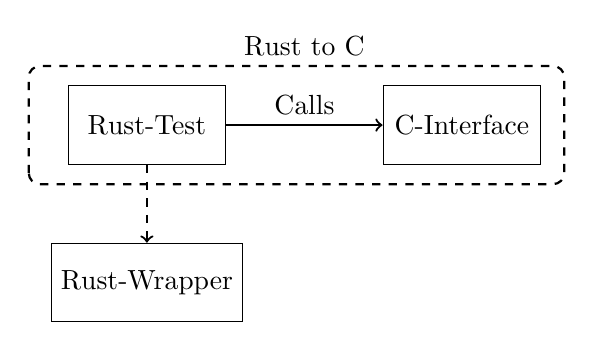
\begin{tikzpicture}asynchronous
  % Nodes
  \node (RS) [rectangle, draw, minimum height=1cm, minimum width=2cm] at (0, 0) {Rust-Test};
  \node (C) [rectangle, draw, minimum height=1cm, minimum width=2cm] at (4, 0) {C-Interface};
  \node (WRAP) [rectangle, draw, minimum height=1cm, minimum width=2cm] at (0, -2) {Rust-Wrapper};
  % Arrows
  \draw[->, thick] (RS) -- (C) node[midway, above] {Calls};
  \draw[->, dashed, thick] (RS) -- (WRAP) node[midway, above] {};
  % Header
  \node (title) at (2, 1) {Rust to C};
  % Dashed lines
  \draw[dashed, thick, rounded corners] (-1.5, -0.75) rectangle (5.3, 0.75);
\end{tikzpicture}

\hfill \break %% newline

%% RS can *use* C results
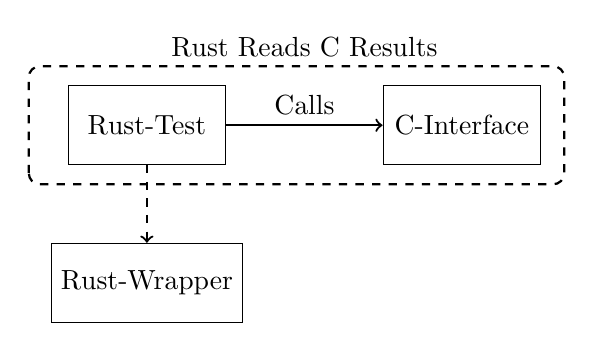
\begin{tikzpicture}asynchronous
  % Nodes
  \node (RS) [rectangle, draw, minimum height=1cm, minimum width=2cm] at (0, 0) {Rust-Test};
  \node (C) [rectangle, draw, minimum height=1cm, minimum width=2cm] at (4, 0) {C-Interface};
  \node (WRAP) [rectangle, draw, minimum height=1cm, minimum width=2cm] at (0, -2) {Rust-Wrapper};
  % Arrows
  \draw[->, thick] (RS) -- (C) node[midway, above] {Calls};
  \draw[->, dashed, thick] (RS) -- (WRAP) node[midway, above] {};
  % Header
  \node (title) at (2, 1) {Rust Reads C Results};
  % Dashed lines
  \draw[dashed, thick, rounded corners] (-1.5, -0.75) rectangle (5.3, 0.75);
\end{tikzpicture}

\hfill \break %% newline

%% Converting C types to Rust types
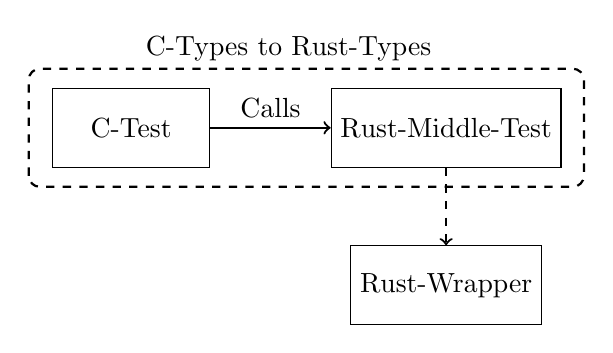
\begin{tikzpicture}asynchronous
  % Nodes
  \node (C) [rectangle, draw, minimum height=1cm, minimum width=2cm] at (0, 0) {C-Test};
  \node (RS-TEST) [rectangle, draw, minimum height=1cm, minimum width=2cm] at (4, 0) {Rust-Middle-Test};
  \node (RS) [rectangle, draw, minimum height=1cm, minimum width=2cm] at (4, -2) {Rust-Wrapper};
  % Arrows
  \draw[->, thick] (C) -- (RS-TEST) node[midway, above] {Calls};
  \draw[->, dashed, thick] (RS-TEST) -- (RS) node[midway, above] {};
  % Header
  \node (title) at (2, 1) {C-Types to Rust-Types};
  % Dashed lines
  \draw[dashed, thick, rounded corners] (-1.3, -0.75) rectangle (5.75, 0.75);
\end{tikzpicture}

\hfill \break %% newline

%% Calling Rust Plugins
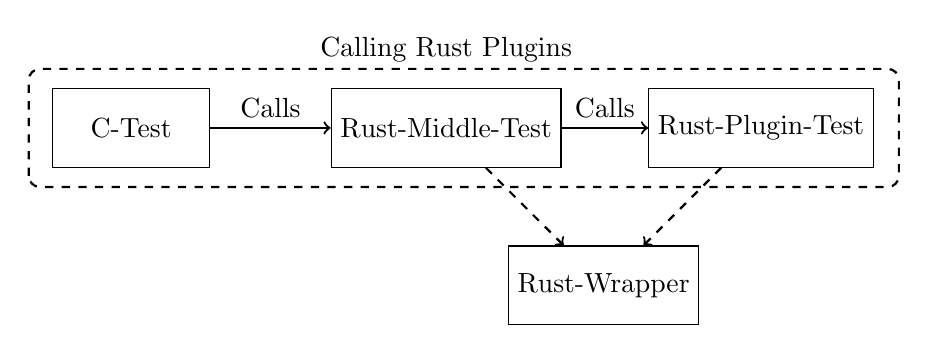
\begin{tikzpicture}asynchronous
  % Nodes
  \node (C) [rectangle, draw, minimum height=1cm, minimum width=2cm] at (0, 0) {C-Test};
  \node (RS-TEST) [rectangle, draw, minimum height=1cm, minimum width=2cm] at (4, 0) {Rust-Middle-Test};
  \node (RS) [rectangle, draw, minimum height=1cm, minimum width=2cm] at (6, -2) {Rust-Wrapper};
  \node (P) [rectangle, draw, minimum height=1cm, minimum width=2cm] at (8, 0) {Rust-Plugin-Test};
  % Arrows
  \draw[->, thick] (C) -- (RS-TEST) node[midway, above] {Calls};
  \draw[->, dashed, thick] (RS-TEST) -- (RS) node[midway, above] {};
  \draw[->, dashed, thick] (P) -- (RS) node[midway, above] {};
  \draw[->, thick] (RS-TEST) -- (P) node[midway, above] {Calls};
  % Header
  \node (title) at (4, 1) {Calling Rust Plugins};
  % Dashed lines
  \draw[dashed, thick, rounded corners] (-1.3, -0.75) rectangle (9.75, 0.75);
\end{tikzpicture}

\hfill \break %% newline

%% Calling * Plugins
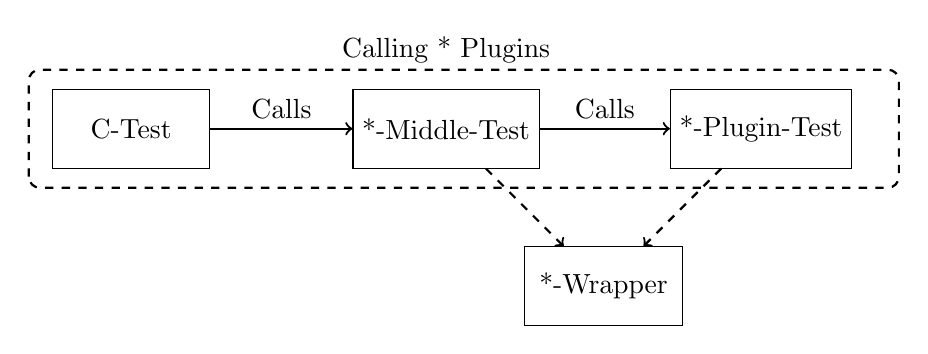
\begin{tikzpicture}asynchronous
  % Nodes
  \node (C) [rectangle, draw, minimum height=1cm, minimum width=2cm] at (0, 0) {C-Test};
  \node (-TEST) [rectangle, draw, minimum height=1cm, minimum width=2cm] at (4, 0) {*-Middle-Test};
  \node (W) [rectangle, draw, minimum height=1cm, minimum width=2cm] at (6, -2) {*-Wrapper};
  \node (P) [rectangle, draw, minimum height=1cm, minimum width=2cm] at (8, 0) {*-Plugin-Test};
  % Arrows
  \draw[->, thick] (C) -- (-TEST) node[midway, above] {Calls};
  \draw[->, dashed, thick] (-TEST) -- (W) node[midway, above] {};
  \draw[->, dashed, thick] (P) -- (W) node[midway, above] {};
  \draw[->, thick] (-TEST) -- (P) node[midway, above] {Calls};
  % Header
  \node (title) at (4, 1) {Calling * Plugins};
  % Dashed lines
  \draw[dashed, thick, rounded corners] (-1.3, -0.75) rectangle (9.75, 0.75);
\end{tikzpicture}




\printbibliography

\end{document}
